%------------------------------------------------------------------------------
%	Setup
%------------------------------------------------------------------------------
\documentclass[journal, twocolumn]{IEEEtran}


\usepackage{graphicx}
\usepackage[breaklinks=true]{hyperref}
\usepackage{amsmath}
\usepackage{multirow}
\usepackage{amssymb}

\usepackage{caption}
\usepackage{subcaption}
\captionsetup{font=footnotesize}

\usepackage{textcase}
\usepackage[tablename=TABLE]{caption}
\DeclareCaptionTextFormat{up}{\MakeTextUppercase{#1}}
\captionsetup[table]{
    labelsep=period,
    justification=centering,
    textformat=up,
}


% correct bad hyphenation here
\hyphenation{op-tical net-works semi-conduc-tor}


\begin{document}
%------------------------------------------------------------------------------
%	Title
%------------------------------------------------------------------------------
\title{An Automatic Face Attendance Checking System using Deep Facial Recognition Technique}


%------------------------------------------------------------------------------
%	Author
%------------------------------------------------------------------------------
\author{Thuy Nguyen-Chinh,
		Thien Do-Tieu,
		Phuong Le-Van-Hoang,
		Sy Nguyen-Tan,
		Qui Nguyen-Van,
		Phu Nguyen-Tan

\thanks{This work is our assignment in the course of "Artificial Intelligence in Control Engineering" Sep-Dec 2018, guided by Dr. Pham Viet Cuong (email: pvcuong@hcmut.edu.vn), Faculty of Electrical and Electronics Engineering, HoChiMinh city University of Technology.}
\thanks{Authors are senior of the Faculty of Electrical and Electronics Engineering, HoChiMinh city University of Technology (e-mail: \{thuy.ng.ch, dotieuthien9997, hpcqt97, tansyab1, nvqui97, tanphu97.nguyen \}@gmail.com).}
\thanks{The software is open source and can be found in \url{https://github.com/AntiAegis/Face-Attendance-System}.}
}


\maketitle


%------------------------------------------------------------------------------
%	Abstract
%------------------------------------------------------------------------------
\begin{abstract}
Nowadays, as computers are powerful enough for implementing complex algorithms, there are numerous applications that people utilize computers to run. In which, facial recognition is one of the most active fields of applications. In fact, computers can not only automatically identify who a person is, but also operate 24/7, which human beings cannot endure. This leads to the replacement of people by computers in some repetitive and real-time applications.

In this work, we apply the facial recognition into an attendance checking system that uses faces of registered people to check their attendance. This system has a GUI which allows easy user-to-system interaction. The core of the system is a deep facial recognition technique, which has four stages (e.g., removing motion-blur frames, detecting faces, removing non-frontal-view faces, and recognizing). Particularly, in the recognition phase, we consider this stage as an open-set facial recognition problem, so the system is able to detect people who have not registered in the database before. Also, we boost the performance of the system by utilizing hardware resources of users' computers. Although the system is designed to run with a low-resolution webcam, its performance is reasonably accurate on our private dataset.
\end{abstract}


\begin{IEEEkeywords}
Face Attendance Checking, Facial Recognition, Deep Learning
\end{IEEEkeywords}


\IEEEpeerreviewmaketitle


%------------------------------------------------------------------------------
%	Introduction
%------------------------------------------------------------------------------
\section{Introduction}
\label{introduction}
%\textbf{This section is of Thien.}
%Introduce about a framework of face recognition system, including face detection, landmark detection, face recognition.

Face recognition systems are applying widely in real life, such as: tracking, managing employees, finding information of ceblerities, etc. There are many approaches to design a face recognition system, but these systems frequently are affected by light, non-frontal faces, resolution of cameras, etc, each method have many separable challenges. Overall, a face recognition has two main stages which are face detection and face recognition, yet we want to create a constraint on frontal faces for users, that lead our system to have three stages: face detection, face landmark detection and face recognition.  
\subsection{Face detection}
Face detection and alignment are essential to many face applications such as face recognition and facial expression analysis. However, the large visual variations of faces, such as occlusions, large pose variations and extreme lightings, impose
great challenges for these tasks in real world applications.

The cascade face detector proposed by Viola and Jones \cite{ref:detect-1} utilizes Haar-Like features and AdaBoost to train cascaded classifiers, which achieve good performance with real-time
efficiency. However, quite a few works [2, 3, 4] indicate that this detector may degrade significantly in real-world applications with larger visual variations of human faces even with more advanced features. Besides the cascade structure, [5, 6, 7] introduce deformable part models (DPM) for face detection and achieve remarkable performance. However, they need high computational expense and may usually require expensive annotation in the training stage. Recently, convolutional neural networks (CNNs) achieve remarkable progresses in a variety of computer vision tasks, especially face detection task. Li et al. [19] use cascaded CNNs for face detection, but it requires bounding box calibration from face detection with extra computational expense and ignores the inherent correlation between facial landmarks localization and bounding box regression. Face alignment also attracts extensive interests. Regression-based methods [12, 13, 16] and template fitting approaches [14, 15, 7] are two popular categories.

However, most of the available face detection and face alignment methods ignore the correlation between these two tasks. Though there exist several works attempt to jointly solve them, there are still limitations in these works. For example, Chen et al. [18] jointly show alignment and detection with random forest using features of pixel value difference. But, the handcraft features used limits its performance. From those previous experiments, we choose an new approach which integrate these two tasks using unified cascaded CNNs by multi-task learning called Multi-task Convolutional Network in section \ref{face-recognition}.
\subsection{Landmark detection}
The locations of the fiducial facial landmark points around facial components and facial contour capture  the  rigid  and  non-rigid  facial  deformations  due to  head  movements  and  facial  expressions.  They  are hence important for various facial analysis tasks. Many facial landmark detection algorithms have been developed to automatically detect those key points over the years. In this paper, we use dlib library which is a powerfull source for face and facial landmark detection. We will discuss our implement in detail in section \ref{frontal-view-detection}.

\subsection{Face recognition}
After face detection and alignment, those regions of face is extracted to get feature vectors. With conventional way, One of the most popular feature for face recognition is Gabor feature. Tudor Barbu ?? uses Gabor transfrom to extract feature, and then using K-Nearest Neighbour (K-NN) based on clustering feature to predict identity of a face. This implement achieve quite impressed performance with accuracy of 90\% on Yale Face Database B. In Opencv library which focuses on algorithms of Computer Vision introduces a method called Local Binary Patterns (LBP) based on Haar-Like feature. In term of speed, LBP has relly real-time efficiency, whereas it is not stable in term of accuracy, this method cannot face with arounded noise which is the reason why LBP and Haar-Like feature are rarely applied in practical systems. Because of limitations of conventional features,  deep learning models gradually instead and get better and better. Yi Sun, Xiaogang Wang, Xiaoou Tang ?? build a deep model Deep hidden IDentity features (DeepID) which uses convolutional neural network to extract face feature. Advantage of this model is using a small dataset for training, that is consideraby good for systems which cannot collect a large dataset of users. However, to reach a high accuracy, DeepID model become really complex with many neural network branches for each person. There are 10 patches of face which contain interested information are chosen from each image, then they are scaled with three figures in RGB and gray chanel. Totally, model have 60 different networks to extact feature of an image, then feedforwarding feature into a classifier using Joint Bayesian. DeepID achieves excellent accuracy of 97.45\% on dataset Labeled Faces in the
Wild (LFW). In 2014, the authors of DeepID show DeepID2 which is a improved version of DeepID. In new version, interested regions of face algorithm is built to eliminate useless patches which cannot extract high-level feature. That work really helpfull affect accuracy, specifically there is a increase in accuracy at 99.63\%. In 2015, Google Inc.?? use deep convolutional network Inception and triplet loss function in FaceNet mdoel to extract feature. Their outstanding work in this model is using hard triplet loss to separate feature for each person, so FaceNet feature is robust in both face verification and face recognition. The accuracy of 99.63\% on LFW and 95.12\% on Youtube Faces
DB dataset is high enough to represent the perfection of model. 
%------------------------------------------------------------------------------
%	Proposed system
%------------------------------------------------------------------------------
\medskip
\section{Proposed system}
\label{proposed-system}

In this paper, we apply deep facial recognition techniques into the problem of face attendance checking. A system is built in order to manage appearances of students in a class. As normally, the system is organized as a pipeline of typical stages, namely face detection, landmark detection, and face recognition. However, to ensure input frames for underlying algorithms are high quality, we append an early filter that are able to discard blur frames, which are caught by motions of people in front of a standard webcam. Besides, we take a more step by adapting the landmark detection to verify whether a face is in frontal view of the camera so that the result of face recognition is more accurate. Also, to leverage the ease in use, the design a friendly graphic user interface (GUI) so that people who want to use the system to manage (teachers) or check (students) attendance can interact with the application without any specific knowledge. To make the system more robust, we carefully analyze the distribution outlier of features representing for registered accounts. Therefore, the algorithm has ability to detect people who have not registered in the application before, which is equivalent to the open-set problem in face recognition. Figure \ref{fig:system} reveals our proposed system.

Our work is organized as follows. In the section \ref{implementation}, stages of the proposed system are described clearly, including motion-blur detection, face detection, frontal-view detection, and face recognition. Then, section \ref{experimental-result} is for reporting some experimental results.


%------------------------------------------------------------------------------
%	Implementation
%------------------------------------------------------------------------------
\medskip
\section{Implementation}
\label{implementation}

\subsection{Motion-blur detection}
\label{motion-blur-detection}
\textbf{This section is of Phu.}

The first stage of this system is detecting blurred image and rejecting them out of next stage. We know that the blurred image means each pixel in the source image gets spread out and mixed into surrounding neighbour pixels. For our attendance checking system, the motion blur happens when an object (namely face or webcam) moves during the exposure. So as to detect whether an image is blurred, we use the 2D-FFT (2D-Fast Fourier Transform) method.

 We will review about Fourier Transform of Images. To compute the Fourier transform of an image, you need to:
\begin{itemize}
\item Compute DFT of each row, in place.
\item Compute DFT of each column, in place.
\end{itemize}  

When a signal is discrete and periodic, we use the discrete Fourier transform, or DFT.
Suppose our signal is $a_n$ for $n=0 \ldots N-1$,
and $a_n=a_{n+jN}$ for all $n$ and $j$.
The spectrum of $a$ is:
\begin{equation}
A_k = \sum_{n=0}^{N-1} W_N^{kn} a_n
\label{dft.eq}
\end{equation}
where
$$
W_N = e^{-i {2 \pi \over N}}
$$
and $W_N^k$ for $k=0 \ldots N-1$ are called the {\it Nth roots of unity}.
The sequence $A_k$ is the discrete Fourier transform of the sequence $a_n$.
Each is a sequence of $N$ complex numbers.

The FFT is a fast algorithm for computing the DFT.
If we take the 2-point DFT and 4-point DFT and generalize them
to 8-point, 16-point, ..., $2^n$-point (n is an integer), we get the FFT algorithm.

There are several ways to write an FFT. For instance, let $m$ be an integer and let $N=2^m$.
Suppose that $x=[x_0,\ldots,x_{N-1}]$ is an $N$ dimensional complex vector.
Let $\omega=\exp({-2\pi i\over N})$.  Then the DFT, $c= F_N(x)$ is given by
\begin{equation}
c_k={1\over N}\sum_{j=0}^{j=N-1}x_j\omega^{jk}.
\end{equation}
Let $n=N/2$, let $u$ and $v$ be $n$ dimensional vectors defined by 
\begin{align}
u_j&=x_j+x_{j+n},\ j=0,\ldots,n-1\\
v_j&=(x_j-x_{j+n})\omega ^j,\ j=0,\ldots,n-1.
\end{align}
Then 
\begin{align}
c_{2j}={1\over 2}(F_n(u))_j,\ j=0,\ldots,n-1\\
c_{2j+1}={1\over 2}(F_n(v))_j,\ j=0,\ldots,n-1.
\end{align}

To compute the DFT of an $N$-point sequence using equation (\ref{dft.eq})
would take $(N^2)$ multiplies and adds.
The FFT algorithm computes the DFT using $(N \log N)$ multiplies and adds.

Practical issues:
We translate the picture so that pixel (0,0), which now contains frequency $(\omega_x,\omega_y)=(0,0)$, moves to the center of the image. Then, we display pixel values proportional to
log(magnitude) of each complex number. For color images, do the above to each of the three channels
(R, G, and B) independently.

Apply to our system, firstly, we calculate FFT of image. Secondly, we will compute mean amplitude spectrum value of entire pixel in image and. Finally, the result of this operation is compared to an optimal threshold which distinguishes blurred and non-blurred image as accurate as possible. The image is called non-blurred if and only if its average value greater than the threshold value, and vice versa. After that, non-blurred images are applied to face detection stage of system.

\subsection{Face detection}
\label{face-detection}
\textbf{This section is of Qui.}

\subsection{Frontal-view detection}
\label{frontal-view-detection}
\textbf{This section is of Qui.}

\subsection{Face recognition}
\label{face-recognition}
%\textbf{This section is of Thien.}
\begin{figure}
    \centering
    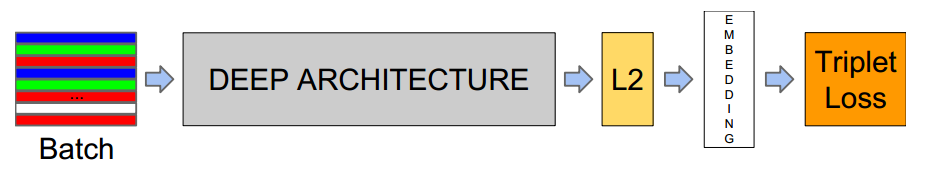
\includegraphics[width=1\linewidth]{img/pipeline.png}
	\caption{Model structure. Our network consists of a batch input layer and a deep CNN 
followed by L2 normalization, which results in the face embedding. This is followed by the triplet loss during training.}\label{fig:pipeline}
\end{figure}

In this stage, faces in raw images are detected and aligned by Multi-task CNN, we use convenient pre-trained FaceNet model to extract feature (in Figure \ref{fig:pipeline}) and then feedforward it to a SVM classifier for regconition. 
\subsubsection{Multi-task Convolution Network}
\begin{figure}
    \centering
    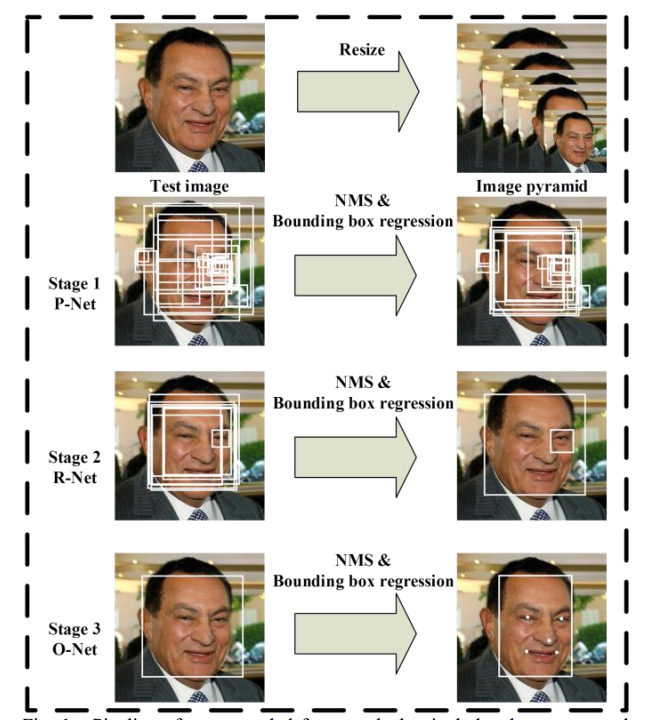
\includegraphics[width=1\linewidth]{img/mtcnn.png}
	\caption{Pipeline of our cascaded framework that includes three-stage multi-task deep convolutional networks. Firstly, candidate windows are produced
through a fast Proposal Network (P-Net). After that, we refine these candidates
in the next stage through a Refinement Network (R-Net). In the third stage,
The Output Network (O-Net) produces final bounding box and facial landmarks position.}\label{fig:mtcnn}
\end{figure}

The overall pipeline Multi-task CNN is shown in Figure \ref{fig:mtcnn}. An image is  initially resized to different scales to build an image pyramid, which is the input of the following three-stage cascaded framework with CNN architectures in Figure \ref{fig:mtcnn-arch}:

\textbf{Stage 1}: A fully convolutional network is exploited, called Proposal Network (P-Net), to obtain the candidate windows and their bounding box regression vectors. Then using the estimated bounding box regression vectors to calibrate the candidates. After that, employing non-maximum suppression (NMS) to merge highly overlapped candidates.

For each candidate window, P-CNN predict the offset between it and the nearest ground truth (i.e.,the bounding boxes’ left top, height, and width). The learning objective is formulated as a regression problem, and  the Euclidean loss is employed for each sample $x_i$:
\begin{align}
	L_i^{box} = \Vert y_i^{prediction} - y_i^{truth} \Vert _2^2
\end{align}
		
\textbf{Stage 2}: All candidates are fed to another CNN, called Refine Network (R-Net), which further rejects a large number of false candidates, performs calibration with bounding box regression, and NMS candidate merge.

\textbf{Stage 3}: his stage is similar to the second stage, but in this stage we aim to describe the face in more details. In particular, the network will output five facial landmarks’ positions.

Similar to the bounding box regression task, facial landmark detection is formulated as a regression problem: 

\begin{align}
	L_i^{landmark} = \Vert y_i^{prediction} - y_i^{truth} \Vert _2^2
\end{align}

\begin{figure}
    \centering
    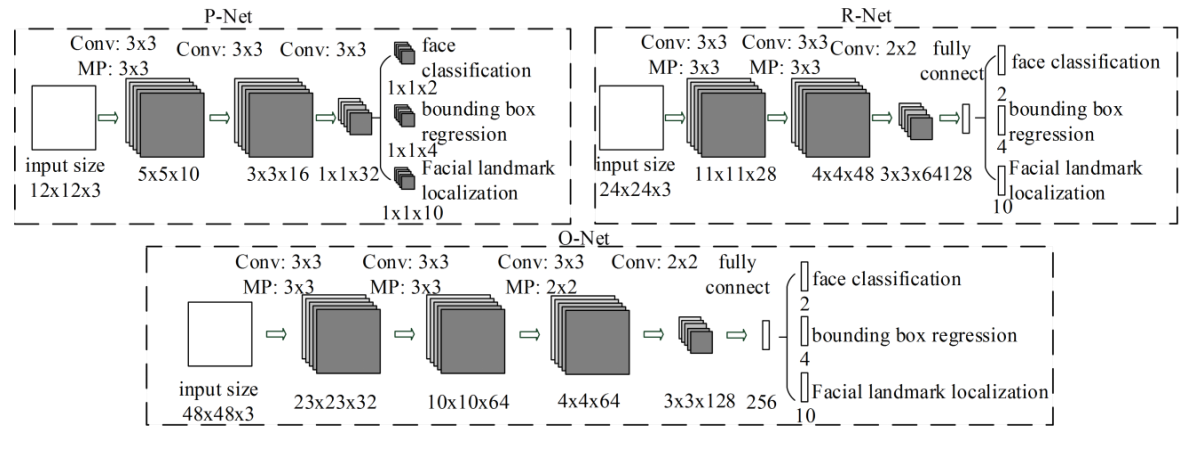
\includegraphics[width=1\linewidth]{img/mtcnn_arch.png}
	\caption{The architectures of P-Net, R-Net, and O-Net, where “MP” means max pooling and “Conv” means convolution. The step size in convolution and pooling
is 1 and 2, respectively}\label{fig:mtcnn-arch}
\end{figure}

\subsubsection{FaceNet model} 
This model use Inception-ResNet v1 architecture ?? and triplet loss to extract feature. Inception-ResNet v1 (in Figure \ref{fig:inception-resnet}) is a very deep convolutional network which combine ResNet network and Inception network with a complex structure. This deep network affords to extract high-level feature for object recognition, and combination with triplet loss gets better and better. 

\begin{figure}
    \centering
    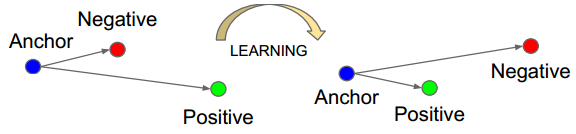
\includegraphics[width=1\linewidth]{img/triplet.png}
	\caption{The Triplet Loss minimizes the distance between an anchor and a positive, both of which have the same identity, and maximizes the distance between the anchor and a negative of a different identity.}
	\label{fig:triplet}
\end{figure}

The embedding is represented by $f(x) \in R^d$. It embeds an image $x$ into a $d$-dimensional Euclidean space. Here we want to ensure that an image $x_i^a$ (anchor) of a specific person is closer to all other images $x_i^p$ (positive) of the same person than it is to any image $x_i^n$ (negative) of any other person. This is visualized in Figure \ref{fig:triplet}. Thus we want, 
\begin{align}
	\Vert f(x_i^a) - f(x_i^p) \Vert_2^2 + \alpha < \Vert f(x_i^a) - f(x_i^n) \Vert_2^2
\end{align}
where $\alpha$ is a margin that is enforced between positive and negative pairs. The loss that is being minimized is then: 
\begin{align}
	L = \sum_i^N(\Vert f(x_i^a) - f(x_i^p) \Vert_2^2  - \Vert f(x_i^a) - f(x_i^n) \Vert_2^2 + \alpha)
\end{align}
In this implement, FaceNet model is trained on VGGFace2 dataset which over 9000 identities and over 3.3 million faces. VGGFace2 is a large-scale face recognition dataset from Google Image Search and have large variations in pose, age, illumination, ethnicity and profession. Therefore, embeddings is specifical for each person. 
\subsubsection{Training} 
To apply Multi-task model and FaceNet model into Face Attandence system, we feedforward raw images of students into Multi-task CNN to get face patches, then extract feature of each patch with 512 dimension vector by pre-trained FaceNet model. After that, we split dataset of students into 3 subsets: training, validating and testing. Each person in training, validating, testing subset contrains 30 images, 10 images and 30 images respectively. We decide to collect only 30 images for training subset, because we want to reduce time of training and time for collecting images. Next, we use SVM classifier to train on trainning subset and validate on validating subset. The output of trained-classifier is probability vector whose each element represent ability of an identity anchor belong to. Thus, anchor is determined by choose which identity have maximum probability, that suffer from mistakes when faces of strangers appear. To solve open-set problem, we combine both two subsets: training and validating to training threshold. This threshold helps us to eliminate unknow people, additionally ensure that the result of system achieve higher accuracy.
\begin{figure}
    \centering
    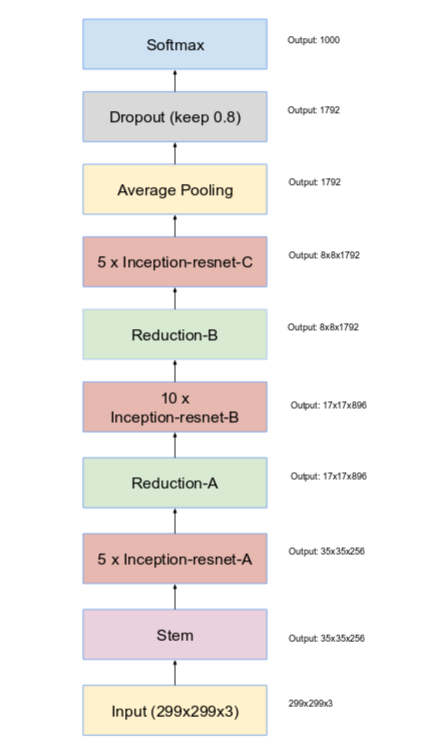
\includegraphics[width=0.7\linewidth]{img/in_res_v1.png}
	\caption{Schema for Inception-ResNet-v1 and Inception-ResNet-v2 networks. This schema applies to both networks but the underlying components differ.}
	\label{fig:inception-resnet}
\end{figure}

\subsection{Graphic User Interface}
\label{gui}
\textbf{This section is of Sy.}


%----------------------------Attendance management-----------------------------
\subsection{Attendance management}
\label{attendance-management}
\textbf{This section is of Phuong.}

This is the final phase of Face Attendance Checking System.
It was designated to mark the presence of one resulted from
our algorithm in a file of excel format, namely xlsx extension.
To be used by the system, the excel file must meet
a stringent format made up of essential contents and be
generated by the GUI. 

Figure \ref{fig:form-new} depicts a new standard empty
excel table generated by our GUI. After obtaining a new file, we should fill in the table with the desired data (Figure \ref{fig:form-data}). The most special things in this table are column ID and Total. 
ID is considered a primary key because the algorithm will mark the presence of a specific person via his ID. 
To help the host in easy attendance management, we designed the column Total with a view to showing the number of absences in all.

Figure \ref{fig:form-checked} depicts an excel file's content after a checking progress finished. 
The GUI will automatically insert the only one new day column between Group and Total ones and in the tail of previous checked day. 
Letter 1 will be marked as presence in a cell of this column accordant to an ID. 
After attendance checking process is completed, the Total column will display the number of absences of previous days and the current one. Smartly can it display as we specially assigned a size-dynamic sum function to each cell of this column.


\begin{figure}
    \centering
    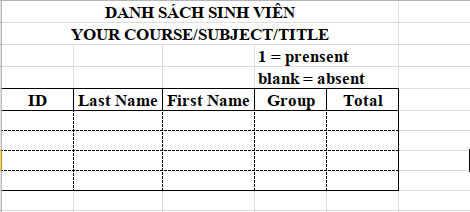
\includegraphics[width=0.8\linewidth]{img/form-new.png}
	\caption{New standard excel form}\label{fig:form-new}
\end{figure}

\begin{figure}
    \centering
    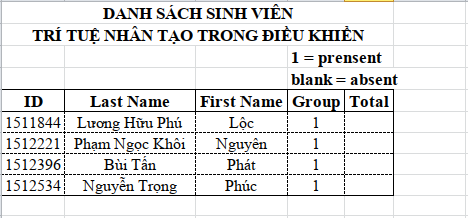
\includegraphics[width=0.8\linewidth]{img/form-data.png}
	\caption{Excel form contain pre-inputed data}\label{fig:form-data}
\end{figure}

\begin{figure}
    \centering
    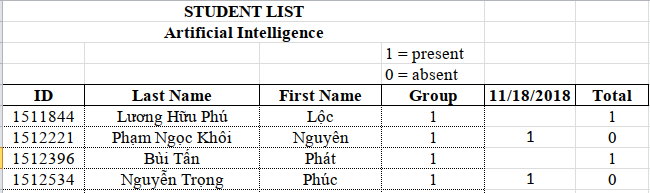
\includegraphics[width=0.8\linewidth]{img/form-checked.png}
	\caption{Form is under checking}\label{fig:form-checked}
\end{figure}


%------------------------------------------------------------------------------
%	Result
%------------------------------------------------------------------------------
\medskip
\section{Experimental result}
In this section, we first evaluate the effectiveness of the feature extracted from FaceNet. Then we will compare our system in different context such as: background, illumination, resolution of camera.Finally, we evaluate the computational efficiency of our system.
\label{experimental-result}
%\textbf{This section is of Thien.}
\subsection{Embedings} 
\begin{figure}[h!]
  \centering
  \begin{subfigure}[b]{0.5\linewidth}
    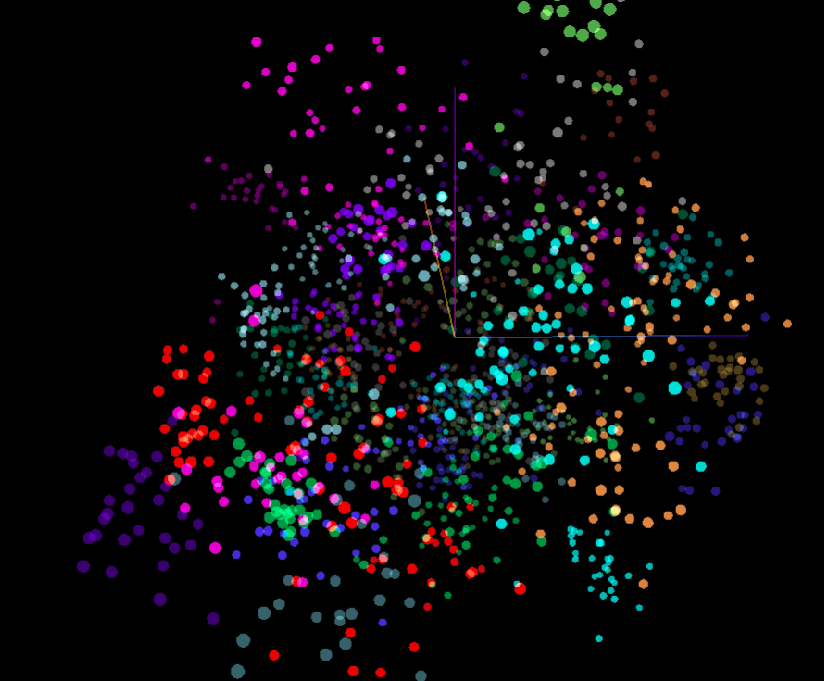
\includegraphics[width=\linewidth]{img/pca1.png}
    \caption{}
  \end{subfigure}
  \begin{subfigure}[b]{0.5\linewidth}
    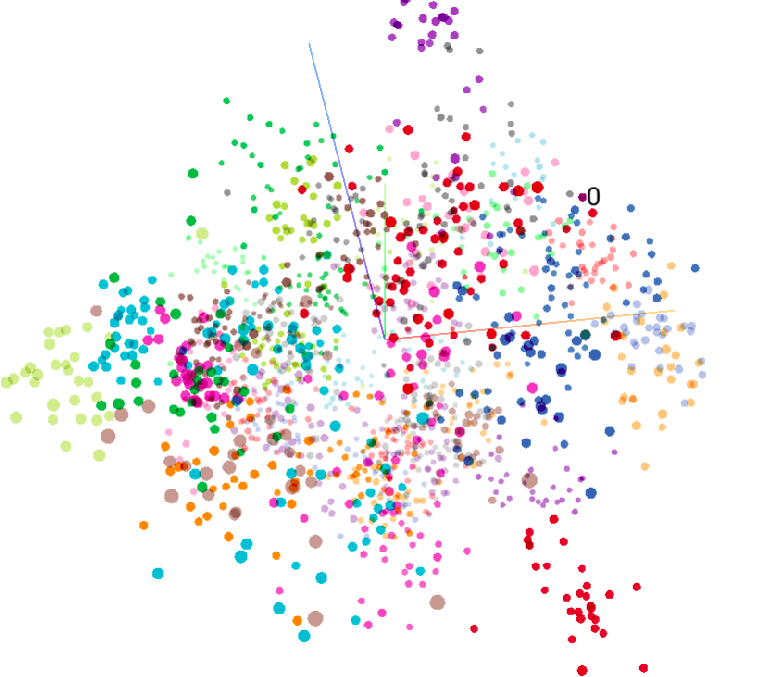
\includegraphics[width=\linewidth]{img/pca2.png}
    \caption{}
  \end{subfigure}
  \begin{subfigure}[b]{0.5\linewidth}
    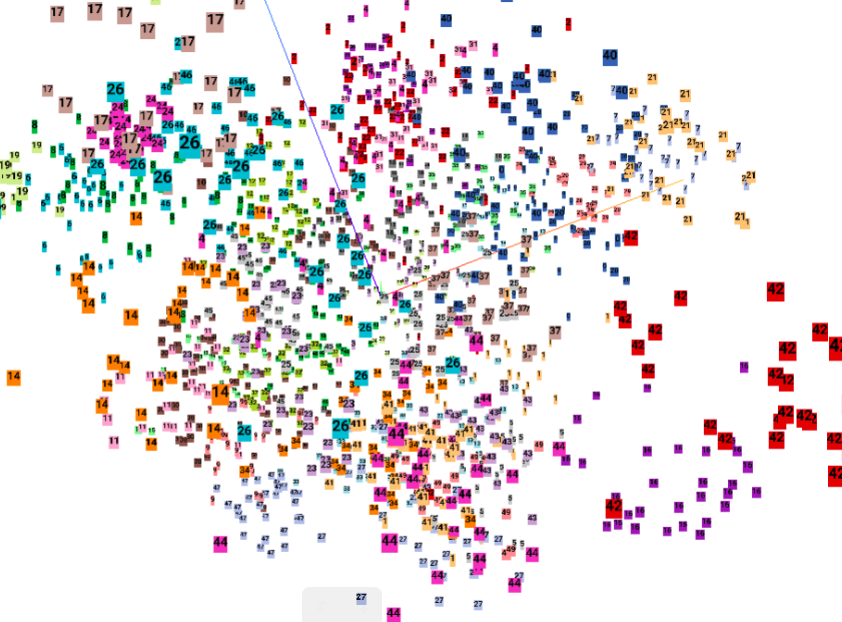
\includegraphics[width=\linewidth]{img/pca3.png}
    \caption{}
  \end{subfigure}
  \caption{Embeddings with PCA visualization} 
  \label{fig:pca}
\end{figure}

\begin{figure}
    \centering
    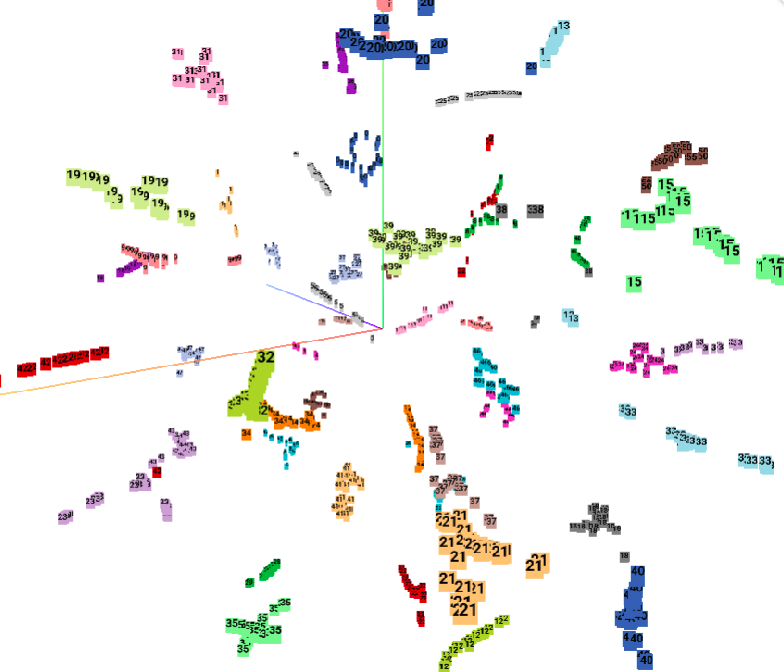
\includegraphics[width=0.7\linewidth]{img/t-sne.png}
	\caption{Embeddings with t-SNE visualization}\label{fig:t-sne}
\end{figure}
Because we use pre-trained model FaceNet, we need to test specification of embeddings which is output of model. We use PCA ?? and t-SNE ?? to visualize embeddings in 3 dimension space in Figure \ref{fig:pca} and Figure \ref{fig:t-sne}. In PCA visualization, embeddings of the same person close together, although they are not completely separable. In another of t-SNE, because t-SNE method include clustering stage, so embeddings totally belong to their classes. If embeddings of FaceNet model is not contain high-level of specification, reducing dimension algorithms cannot show or cluster embeddings properly.  
\subsection{Training}
Training data is carefully collected with different views from $-70^\circ$ to $70^\circ$. This work can improve accuracy in pratical system ,because it is difficult for users to keep their faces in a correct position. In training data include 52 identities and 1560 images totally.

The accuracy of SVM classifier is 99.36\%, after training classifier, we train to get the best threshold. We divide threshold in range $[0;1]$ with .As a result, threshold for 52 identities is 0.18825. Testing accuracy with threshold achieve 98.85\% on testing subset. In practical environment, we test on 32 identities, three are 29 identites recognized easily and 3 identities who are not recognized continuously. In Figure \ref{fig:compare}, the (a),(b) are training images and (c),(b) are testing images, the effect of different ilumination lead the probabilities of testing anchor are lower than threshold, so training data have to cover many real-life cases to create the best classifier.  

\begin{figure}[h!]
  \centering
  \begin{subfigure}[b]{0.35\linewidth}
    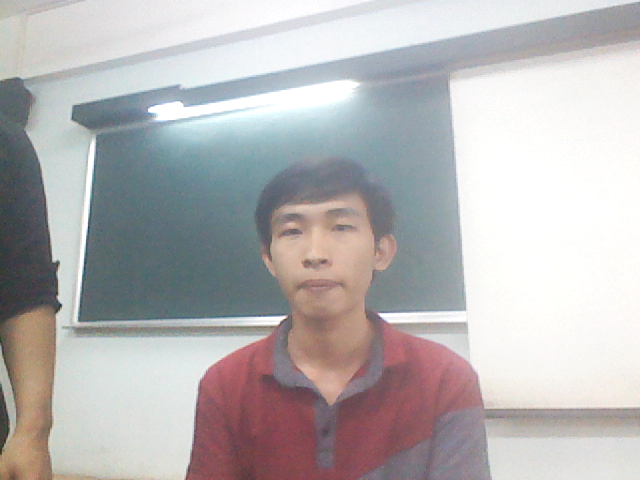
\includegraphics[width=\linewidth]{img/1.png}
    \caption{}
  \end{subfigure}
  \begin{subfigure}[b]{0.35\linewidth}
    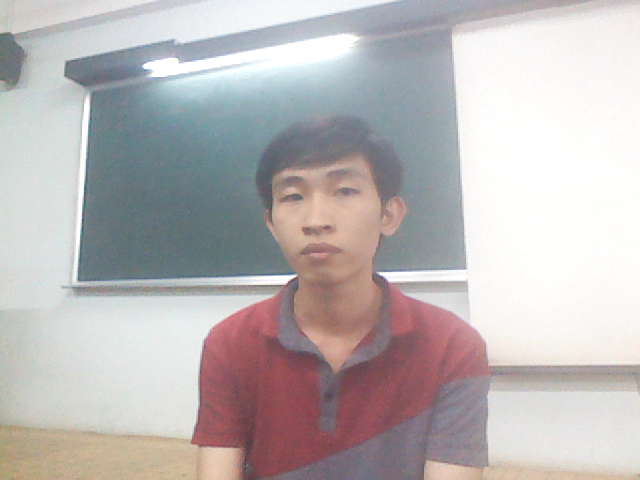
\includegraphics[width=\linewidth]{img/2.png}
    \caption{}
  \end{subfigure}
  \begin{subfigure}[b]{0.35\linewidth}
    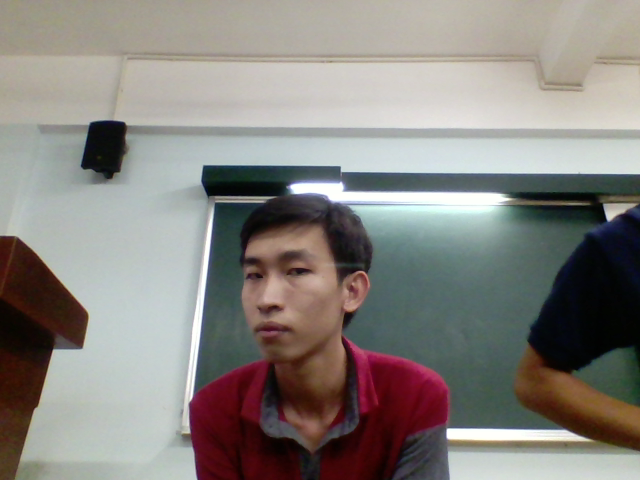
\includegraphics[width=\linewidth]{img/3.png}
    \caption{}
  \end{subfigure}
    \begin{subfigure}[b]{0.35\linewidth}
    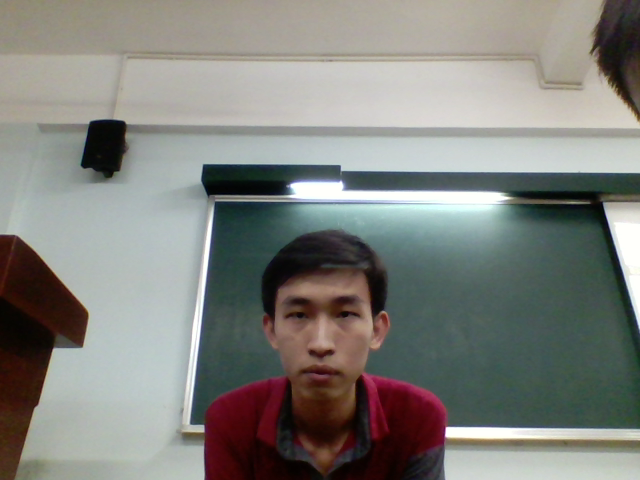
\includegraphics[width=\linewidth]{img/4.png}
    \caption{}
  \end{subfigure}
  \caption{Unrecognized identity, (a),(b) are training images, and (c),(d) are testing images in pratical condition.} 
  \label{fig:compare}
\end{figure}


%------------------------------------------------------------------------------
%	Conclusion
%------------------------------------------------------------------------------
\medskip
\section{Conclusion}
\label{conclusion}

In this work, we applied the deep facial recognition techniques to solve the problem of face attendance checking. The system has a pipeline with four stages (e.g., motion-blur detection, face detection, landmark detection, and face recognition). Besides, the system is also integrated a friendly GUI, which allows users both teachers and students interact with it in an easy way. On our private dataset, the application perform accurate despite of the low-resolution webcam of typical laptops. This demonstrates that our underlying algorithm is effective to deal with this poor-quality input problem.

In the future, we will target to widen our dataset so that the dataset will be asymptotic to real applications. In addition, more algorithms will be considered to improve the ability of the algorithm to discriminate feature distributions of output classes.


%------------------------------------------------------------------------------
%	Acknowledgment
%------------------------------------------------------------------------------
\section*{Acknowledgment}

The authors would like to thank Dr. Pham Viet Cuong for providing documents as well as chance for us to do this work. Also, the authors would like to thank ...


%------------------------------------------------------------------------------
% References
%------------------------------------------------------------------------------
\begin{thebibliography}{9}
%% Copy-Move-------------------------------------------------------------------
%%%% Key-point-based
\bibitem{ref:keypoint-1}
X. Pan and S. Lyu,
\textit{``Region duplication detection using image feature matching"},
IEEE Transactions on Information Forensics and Security,
vol. 5, no.4, ISSN: 1556-6013, pp. 857-867, 2010.
	
\bibitem{ref:keypoint-2}
I. Amerini, L. Ballan, R. Caldelli, A. Del Bimbo and G.Serra,
\textit{``A sift-based forensic method for copy–move attack detection and transformation recovery"},
IEEE Transactions on Information Forensics and Security,
vol. 6, no. 3, ISSN: 1556-6013, pp. 1099-1110, 2011.

\bibitem{ref:keypoint-3}
P. Kakar, N. Sudha,
\textit{``Exposing postprocessed copy-paste forgeries through transform-invariant feature"},
IEEE Transactions on Information Forensics and Security,
vol. 7, no. 3, ISSN: 1556-6013, pp. 1018-1028, June 2012.

%%%% Block-based
\bibitem{ref:block-1}
S.-J. Ryu, M.-J. Lee and H.-K. Lee,
\textit{``Detection of copy-rotate-move forgery using Zernike moments"},
Information Hiding Conference, Lecture Notes in Computer Science, vol. 6387, Springer,
Heidelberg-Berlin, 2010, ISBN: 978-3-642-16434-7.

\bibitem{ref:block-2}
H.-J. Lin, C.-W. Wang and Y.-T. Kao,
\textit{``Fast copy-move forgery detection"},
WSEAS Transactions on Signal Processing,
vol. 5, no. 5, ISSN: 0031-3203, pp. 188-1975, 2009.

\bibitem{ref:block-3}
V. Christlein, C. Riess, J. Jordan and E. Angelopoulou,
\textit{``An evaluation of popular copy-move forgery detection approaches"},
IEEE Transactions on Information Forensics and Security,
vol. 7, no. 6, ISSN: 1556-6013, pp. 1841-1854, 2012.

\bibitem{ref:block-4}
T. L.-Tien, T. H.-Kha, L. P.-C.-Hoan, A. T.-Hong, N. Dey, M. Luong,
\textit{``Combined Zernike Moment and Multiscale Analysis for Tamper Detection in Digital Images"},
Informatica (An International Journal of Computing and Informatics),
vol.41, no.1, ISSN: 0350-5596, March 2017.


%% JPEG format-----------------------------------------------------------------
\bibitem{ref:jpeg-dct-1}
Z. Lin, J. He, X. Tang, K. Tang,
\textit{``Fast, automatic and fine-grained tampered JPEG image detection via DCT coefficient analysis"},
Pattern Recognition, vol. 42, no. 11, ISSN: 0031-3203, pp. 2492-2501, January 2009.

\bibitem{ref:jpeg-dct-2}
W. Wang, J. Dong, T. Tan,
\textit{``Exploring DCT coefficient quantization effects for local tampering detection"},
IEEE Transactions on Information Forensics and Security,
vol. 9, no. 10, ISSN: 1556-6013, pp. 1653-1666, October 2014.

\bibitem{ref:jpeg-periodicity}
L. Chen, T. Hsu,
\textit{``Detecting recompression of JPEG images via periodicity analysis of compression artifacts for tampering detection"},
IEEE Transactions on Information Forensics and Security,
vol. 6, no. 2, ISSN: 1556-6013, pp. 396-406, June 2011.

\bibitem{ref:jpeg-improved}
L. Thing, Y. Chen, C. Cheh,
\textit{``An improved double compression detection method for JPEG image forensics"},
In IEEE International Symposium on Multimedia,
pages 290-297, December 2012, ISBN: 978-1-4673-4370-1.

\bibitem{ref:jpeg-ghosts}
F. Zach, C. Riess, and E. Angelopoulou,
\textit{``Automated image forgery detection through classification of JPEG ghosts"},
Pattern Recognition, 7476, pp. 185-194, January 2012.

\bibitem{ref:jpeg-block-grained}
T. Bianchi, A. Piva,
\textit{``Image forgery localization via block-grained analysis of JPEG artifacts"},
IEEE Transactions on Information Forensics and Security,
vol. 7, no. 3, ISSN: 1556-6013, pp. 1003-1017, June 2012.

\bibitem{ref:jpeg-inpainting}
C. Chang, C. Yu, C. Chang,
\textit{``A forgery detection algorithm for exemplar-based inpainting images using multi-region relation"},
Journal Image and Vision Computing,
vol. 31, no. 1, ISSN: 0262-8856, pp. 57-71, MA-USA, 2013.


%% Deep Learning approach------------------------------------------------------
\bibitem{ref:cnn-median}
J. Chen, X. Kang, Y. Liu and Z. J. Wang,
\textit{``Median Filtering Forensics Based on Convolutional Neural Networks"},
IEEE Signal Processing Letters,
vol. 22, no. 11, ISSN: 1070-9908, pp. 1849-1853, November 2015.

\bibitem{ref:cnn-universal}
B. Bayar, M. C. Stamm,
\textit{``A Deep Learning Approach to Universal Image Manipulation Detection Using a New Convolutional Layer"},
Proceedings of the 4th ACM Workshop on Information Hiding and Multimedia Security,
pp. 5-10, New York-USA, 2016, ISBN: 978-1-4503-4290-2.

\bibitem{ref:cnn-srm}
Rao Yuan, Ni Jiangqun,
\textit{``A deep learning approach to detection of splicing and copy-move forgeries in images"},
IEEE International Workshop on Information Forensics and Security (WIFS),
Abu Dhabi-United Arab Emirates, 2016, ISBN: 978-1-5090-1139-1.

\bibitem{ref:cnn-alex}
J.Ouyang, Y.Liu, M.Liao,
\textit{``Copy-Move Forgery Detection Based on Deep Learning"},
10th International Congress on Image and Signal Processing, BioMedical Engineering and Informatics,
Shanghai-China, 2017, ISBN: 978-1-5386-1938-4.

\bibitem{ref:dae}
Y. Zhang, J. Goh, L. Win, V. Thing,
\textit{``Image Region Forgery Detection: A Deep Learning Approach"},
Proceedings of the Singapore Cyber-Security Conference, Singapore, 2016, ISBN: 978-1-61499-616-3.


%% Database--------------------------------------------------------------------
\bibitem{ref:casia}
J. Dong and W. Wang,
\textit{``Casia tampering detection dataset"}, 2011.


%% Machine Learning------------------------------------------------------------
\bibitem{ref:alex-net}
A. Krizhevsky, I. Sutskever, G. Hinton,
\textit{``Imagenet classification with deep convolutional neural networks"},
NIPS'12 Proceedings of the 25th International Conference on Neural Information Processing Systems,
vol. 1, pp. 1097-1105, Nevada-USA, 2012, DOI: 10.1145/3065386.

\bibitem{ref:dropout}
N. Srivastava, 	G. Hinton, A. Krizhevsky, I. Sutskever, R. Salakhutdinov,
\textit{``Dropout: a simple way to prevent neural networks from overfitting"},
The Journal of Machine Learning Research,
vol. 15, no. 1, ISSN 1533-7928, pp. 1929-1958, January 2014.

\bibitem{ref:xavier}
Xavier Glorot, Yoshua Bengio,
\textit{``Understanding the difficulty of training deep feedforward neural networks"},
Proceedings of the 13rd International Conference on Artificial Intelligence and Statistics,
PMLR 9, pp. 249-256, Sardinia-Italy, \url{http://proceedings.mlr.press/v9/glorot10a/glorot10a.pdf}, 2010.

\bibitem{ref:relu}
V. Nair, E. Hinton,
\textit{``Rectified Linear Units Improve Restricted Boltzmann Machines"},
Proceedings of the 27th International Conference on Machine Learning,
pp. 807-814, Haifa-Israel, 2010, ISBN: 978-1-60558-907-7.

\bibitem{ref:leaky-relu-1}
B. Xu, N. Wang, T. Chen, M. Li,
\textit{``Empirical Evaluation of Rectified Activations in Convolutional Network"},
\url{https://arxiv.org/abs/1505.00853v2}, 2015.

\bibitem{ref:leaky-relu-2}
K. He, X. Zhang, S. Ren, J. Sun
\textit{``Delving Deep into Rectifiers: Surpassing Human-Level Performance on ImageNet Classification"},
\url{https://arxiv.org/abs/1502.01852v1}, 2015.

\bibitem{ref:adam}
P. Kingma, J. Ba,
\textit{``Adam: A Method for Stochastic Optimization"},
3rd International Conference for Learning Representations, San Diego-USA,
\url{https://arxiv.org/abs/1412.6980}, 2015.


%% Comparison------------------------------------------------------------------
\bibitem{ref:goh}
J. Goh and V. L. L. Thing,
\textit{``A hybrid evolutionary algorithm for feature and ensemble selection in image tampering detection"},
International Journal of Electronic Security and Digital Forensics,
vol. 7, no. 1, ISSN: 1751-911X, pp. 76-104, March 2015.

\bibitem{ref:he}
Z. He, W. Lu, W. Sun, J. Huang,
\textit{``Digital image splicing detection based on Markov features in DCT and DWT domain"},
Pattern Recognition, vol. 45, no. 12, ISSN: 0031-3203, pp. 4292-4299, 2012.


%% Appendix--------------------------------------------------------------------
\bibitem{ref:prove-wavelet}
A. Cohen, T. Tiplica, and A. Kobi,
\textit{``Design of experiments and statistical process control using wavelets analysis"},
Control Engineering Practice,
vol. 49, ISSN: 0967-0661, pp. 129-183, April 2016.


\end{thebibliography}

\end{document}